% Overture Language Manual
\documentclass{overturerepchap}
\usepackage{url}
\usepackage{graphics}
\usepackage{times}
\usepackage{listings}
\usepackage{color}
\usepackage{graphicx}
\usepackage{latexsym}
\usepackage{longtable} % ,multirow
\usepackage{makeidx}
\usepackage{hyperref}
\usepackage{ifthen}
\usepackage{makeidx}
\usepackage{fancyhdr}
\usepackage{qtree}


\pagestyle{fancy}
\fancyhead{}
\fancyhead[LO]{\leftmark}
\fancyhead[RE]{VDM-10 Language Manual}
\fancyhead[RO,LE]{\resizebox{0.05\textwidth}{!}{\includegraphics{logo.jpg}}}
\fancyfoot[C]{\thepage}
\makeindex

\begin{document}
 
\title{VDM-10 Language Manual}
\author{ Kenneth Lausdah \and Augusto Ribeiro}

\date{August 2011}
\reportno{TR-002}     

\pagenumbering{roman}
\maketitle


{\textbf{Document history}}

\begin{tabular}{|l|l|l|l|}\hline
Month   & Year & Version \\ \hline
April   & 2010 &    \\ \hline
\end{tabular}

%\addtocounter{page}{2}
\tableofcontents
\newpage
\mbox{}
\newpage
\pagenumbering{arabic} 
\setcounter{page}{1}

\chapter{Introduction}
In order to achieve an ideal common AST three goals have been identified:
\begin{enumerate}
\item \textit{Development must be supported both at specification and implementation level, allowing the VDM language itself to be used for tool specification.}
\item \textit{The AST must be extensible while extensions must be kept isolated within a plug-in.}
\item \textit{Sufficient navigation machinery must exist for an editor so that features like e.g. completion and re-factoring can be implemented easily.}
\end{enumerate}
The following subsections will explain the essential principles for the new AST and what changes are required to a generator in order to produce an AST that complies with the identified goals.




It is essential that a new AST is easy to maintain and easy to extend, thus it must only contain functionality essential for the tree structure. To achieve both easy maintenance and support for specification and implementation level development an abstract tree definition can be used like in the \texttt{ASTGen} tool. However, extendibility is another matter that need attention; This can be handled by allowing one tree to extend another, by adding new nodes and fields or even refining a type of an existing field.





% !TeX root = AstCreator.tex
\definecolor{dkgreen}{rgb}{0,0.6,0}
\definecolor{gray}{rgb}{0.5,0.5,0.5}
\definecolor{mauve}{rgb}{0.58,0,0.82}
\lstnewenvironment{astlst}[1][]%
{\lstset{basicstyle=\footnotesize\ttfamily,language=Java, morekeywords={Packages,Tokens,Abstract,Syntax,Tree,Aspect,Declaration},frame=single,stringstyle=\color{mauve},commentstyle=\color{dkgreen}}#1}
{}



\section{Syntax}

The new AST that has been developed has an improved structure compared to both the existing Overture and VDMJ trees. The main addition made here is the ability to extend an AST while keeping the changes isolated in a plug-in architecture, explained in detail in section~\ref{sec:astExtendIsolation}. Secondly, the AST is specified using a grammar file inspired by SableCC\footnote{\url{http://www.sablecc.org/}}, and can generated to both VDM and Java as supported by \texttt{ASTGen}. The main structural change compared to the Overture AST is the ability to add fields to super classes.








The syntax is divided into a number of sections:

\begin{description}

\item[\textbf{\texttt{Packages}}] This section allowed the default packages to be defined for \texttt{base} that forms the basis for all nodes if nothing else is specified and \texttt{analysis} where all visitors will be generated under:

\begin{astlst}
Packages
base org.overture.ast.node;
analysis org.overture.ast.analysis;
\end{astlst}


\begin{figure}[h]

  \centering
    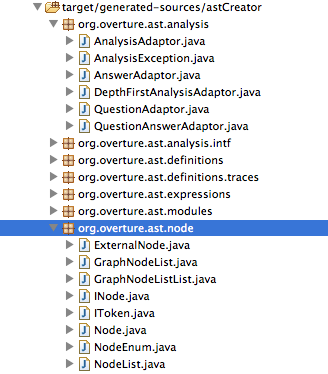
\includegraphics[width=0.5\textwidth]{figures/packageOutput}
      \caption{The package structure of the generated example.}
\end{figure}

\item[\textbf{\texttt{Tokens}}] This section defines tokens or external nodes that can be used as fields in the AST. \textit{The important part here is that they must be clonable}. Tokens  are non-generated classes which are used by the generated nodes. Tokens can be used as fields of AST Nodes and are Java classes. The following types of tokens can be specified:
\begin{description}
\item [Token] A token is an instance of the class \texttt{Token}, it is automatically generated from a name plus the text it represents.

\item [Standard Java Types] Standard Java types (basic types) can be used in the class form. These tokens start with the keyword \texttt{java:}. The use of those relies on them being passed by value when cloning is done. E.g. \texttt{Integer, Boolean, Long, Character, ...}

\item [External Java enum] This is like the standard Java type where the type given is a Java \texttt{enum}.  These tokens start with the keyword \texttt{java:enum:}

\item [External classes] Any external class can be used as a field in the AST but it must implement the interface \texttt{ExternalNode} that provides a handle to the AST for proper cloning for the node.  These tokens start with the keyword \texttt{java:}

\item [External defined Node] This enables a node to be specified outside the AST creator but still included in the analysis. The class must extend \texttt{Node} and do a proper implementation of the analysis methods and kind methods returning the correct enumeration.  These tokens start with the keyword \texttt{java:node:}

\end{description}

\begin{astlst}
Tokens
//Token 
bool = 'bool'; 
//Standard Java Type
java_Integer = 'java:java.lang.Integer'; 
//External Java enum
nameScope = 'java:enum:org.overturetool.vdmj.typechecker.NameScope';
//External Java type
location = 'java:org.overturetool.vdmj.lex.LexLocation'; 
//External defined node
LexToken = 'java:node:org.overturetool.vdmj.lex.LexToken'; 
\end{astlst}

\item[\texttt{Abstract Syntax Tree}] This section describes the tree. Names at the top level are considered roots and \# are considered sub roots. Sub roots must be  specified as a root and a child. 

\begin{astlst}
Abstract Syntax Tree
exp {-> package='org.overture.ast.expressions'}
    =   {binary} [left]:exp [op]:binop [right]:exp
    |   ...
    ;

binop {-> package='org.overture.ast.expressions'}
    = {and}
    |   {or}
    |   ...
    ;
\end{astlst}


%#Unary {-> package='org.overture.ast.expressions'}
%    =   {absolute} 
%    |   {head} 
%    |   {mapInverse} (mapType):type.#Map
%    ;

The above example will generate a tree like:
\begin{figure}[htb]
\begin{minipage}{0.5\linewidth}

\texttt{
\Tree[.exp [.binary left:exp op:binop right:exp ] ]}
\caption{AST Example.}

\end{minipage}
\begin{minipage}{0.5\linewidth}

\texttt{
\Tree[.PExp [.ABinaryExp left:PExp op:PBinop right:PExp ] ]}
\caption{AST Java Generated code Example.}

\end{minipage}
\end{figure}

\begin{description}
\item [The type of field]:
Fields can be specified in two different ways:
\begin{description}
\item[Tree]: Tree fields are fields that belong to a single node in tree and only that one. A tree node cannot be a child of any other node in the tree. Thus if an instance is assigned to a tree field the parent it may belong to is disconnected such that the child/parent relation ship is preserved.\\
Tree fields are syntactically specified as: \texttt{[feld]:type}, where \texttt{field} is the name and \texttt{type} is the type name.
\item[Graph]: Graph fields are reference fields thus the get parent will not deterministically return a single parent but just the first parent the instance was added as a reference field of. This type of node can e.g. be used to add type information to nodes where the type is a reference to a shared type. \\
Tree fields are syntactically specified as: \texttt{(field):type}, where \texttt{field} is the name and \texttt{type} is the type name.
\end{description}

\item [Field types]:
Fields must define the type of the field as a name reference to a tree element like shown in listing~\ref{} above. The syntax is \texttt{:type} where the type can be any of the below shown references:
\begin{description}
\item[Simple types]: Simple types is just the type name like \texttt{:exp} or if a nested type is given \texttt{exp.\#unary.abs}
\item[Lists]: Lists are specified as simple types but appended with a star \texttt{:exp*}
\item[Double lists]: List simple types but with two stars \texttt{:exp**}
\end{description}

\item [Sub-classing]: A sub class can be made by specifying a root as an alternative of another root. The naming convention dictates that the sub class roots must begin with \#. See Figures \ref{fig:ASTExample} and \ref{fig:ASTJavaExample}


\begin{figure}[htb]
\begin{minipage}{0.5\linewidth}

\texttt{
\Tree[.exp \#unary ]}
\\
and
\\

\texttt{
\Tree[.\#unary abs minus ]}
\caption{AST Example.}
\label{fig:ASTExample}
\end{minipage}
\begin{minipage}{0.5\linewidth}

\texttt{
\Tree[.PExp [.SUnaryExp AAbsUnaryExp AMinusUnaryExp ] ]}
\caption{AST Java Generated code Example.}
\label{fig:ASTJavaExample}
\end{minipage}
\end{figure}

\end{description}

\item[\textbf{\texttt{Aspect Declaration}}] This is a feature that allows any fields to be added to base classes (root classes in the AST grammar, the nodes where a a package can be specified). One example could be to add a \texttt{location} field to all nodes of the \texttt{exp} type. The field will be the first declared field in any of the sub classes of \texttt{exp}. The syntax looks like this:

\begin{astlst}
Abstract Declaration
%exp = [location]:location
    ;
\end{astlst}
Where \% prefixes the root node name. The name can also be a composite name like \texttt{\%exp.\#unary}.

\end{description}

\section{Node's ``toString"}

The toString macro-processing enables nodes to have a custom toString to make debugging easier. The  AST is generated with a toString function that prints all fields one after another. However, in some cases debugging might be eased by printing the node in a more suitable format (e.g. in the syntax of the language at hand). To allow such customization a macro-processor is available together with a small language.

The base princiles is that all fields of a node is accessed as defined in the AST e.g. field 1 is accessed through [field1] and strings can be added around the fields by a quoted test ''example test''. The custom toString is defined per node by \%node->sub1 = and can only be defined for leafs of the tree (\textbf{A}-nodes). Furthermore, it is possible to embed java withing the toString by using \$ to escape to java. If external java classes are to be used withing the toString any imports that might be used must be specified in the begining of the file with the \texttt{\textbf{import}} keyword as shown below:

\begin{lstlisting}[language=java,tabsize=2,basicstyle=\ttfamily\footnotesize]
To String Extensions
// import packages used by external $$ java code
import org.overture.ast.util.Utils;
import org.overture.ast.util.ToStringUtil;


//  Expressions

%exp->apply = [root] "(" + $Utils.listToString($ [args] $)$ + ")"
\end{lstlisting}






\section{Analysis}

The generator automatically generated a number of  visitors that can be applied to any node in the ast, those are:

\begin{itemize}
\item Analysis: Simple visitor.
\item Answer: Simple visitor that allows a return value.
\item Question: Simple visitor that allows an argument to be parsed along.
\item QuestionAnswer: Simple visitor that allows an argument to be parsed along and a return value to be returned.
\item DepthFirstAnalysis: Same as Analysis but does a depth first visit of the tree. All fields are visited for each node in the specified order from the syntax, base classes first.
\end{itemize}

All visitors define methods that can be overridden if needed. The methods are named based on the type of node:
\begin{itemize}
\item Simple alternatives: \texttt{caseA} followed by the name of the alternative.
\item Sub roots (prefixed in the gramme with \# and \texttt{S} in the generated class): \texttt{defaultS} the name of the sub root
\item Roots (prefixed \texttt{P} in the generated class): \texttt{defaultP} the name of the root
\end{itemize} 

The following listing illustrates how an overridden method for an unary interpreter van be implemented. It makes use of the numeration kind of the unary operator identifying the sub class of operator hold by the \texttt{node.getOperator()} field. This way all subclasses can be auto inserted in a switch statement by e.g. Eclipse.

\lstset{language=Java,basicstyle=\footnotesize\ttfamily}
\begin{lstlisting}
@Override
public Value caseAUnaryExp(AUnaryExp node)
{
	Value val = node.getExp().apply(this);
	switch (node.getOperator().kindPUnop())
	{
		case ABS:
			return new DoubleValue(val);
		case MINUS:
			return new DoubleValue(val);
		}
	return new BooleanValue(false);
}
\end{lstlisting}


\section{Usage}
The ast generator can be invokes like: 

\begin{astlst}
java -cp astCreator.jar com.lausdahl.ast.creator.CmdMain ast.astV2 .
\end{astlst}

\subsection{Invoking AST Creator using Maven}

The AST Creator is made available as a maven plug-in that enables an AST to be automatically build as part of the build process. The current plug-is in avaliable in the overture repo at: \url{http://build.overturetool.org/builds/mt4e-m2repo-eclipse3.7.2/}

The plug-in is:

\begin{tabular}{ |l|l| }\hline
  groupId & org.overturetool.tools\\\hline
artifactId &astcreatorplugin\\\hline
version & 1.0.6\\\hline
\end{tabular}

The astcreatorplugin plug-in has the goal \textbf{generate} for AST generation and the following configuration properties:

\begin{description}
\item[deletePackageOnGenerate] A list of java packages that should be deleted before generation
\item[ast] A path to the ast file starting from src/main/resources
\item[outputDirectory] an option to define an alternative output location for the generated AST
\end{description}

The pom configuration is as shown below in listing~\ref{}.

\begin{lstlisting}[language=XML,tabsize=2,basicstyle=\ttfamily\footnotesize]
<build>
		<plugins>
			<plugin>
				<groupId>org.overturetool.tools</groupId>
				<artifactId>astcreatorplugin</artifactId>
				<version>1.0.6</version>
				<executions>
					<execution>
						<id>java</id>
						<phase>generate-sources</phase>
						<goals>
							<goal>generate</goal>
						</goals>
					</execution>
				</executions>
				<configuration>
					<deletePackageOnGenerate>
						<param>vdm.generated.node</param>
						<param>org.overture.ast</param>
					</deletePackageOnGenerate>
					<ast>overtureII.astv2</ast>
					<!--outputDirectory>${project.basedir}/src/main/java</outputDirectory -->
				</configuration>
			</plugin>
		</plugins>
\end{lstlisting}


\section{Extensions}

%\subsection{Extendibility and Isolation of Additions}\label{sec:astExtendIsolation}

%\begin{itemize}
%\item The general idea about creating a new grammar file and adding only the new stuff, new fields and nodes.
%\item First proposal isolate changes and make a new AST. Not a good idea. No reuse at all
%\item Solution creating a new subclassed AST with the additions.
%\item Create
%\end{itemize}

In this subsection we describe a new way to specify and generate a tree that extends a base tree and preserves backwards compatibility with its base tree. Extensions are only visible to components that depend on the extended tree otherwise only the base tree structure will be accessible. In figure~\ref{fig:ast_extensions} examples of extensions required by Overture is shown. Each box defines a plug-in feature that needs its own extensions like a type field to store the derived type information from a type checker and a proof obligation generator needs a place to attach proof obligations. The figure also illustrates that an extended tree may be further extended; In this case the derived type information is needed by the interpreter. 

\begin{figure}[tbh]
\centering
\includegraphics[width=.4\textwidth]{figures/ast_extensions}
\caption{Illustration of AST extensions in Overture.\label{fig:ast_extensions}}
\end{figure}

The extension principle is based on sub-classing from a class-hierarchy where each extended node sub-classes the corresponding node in the base hierarchy. This allows a new extended AST to be used by any implementation that supports its base tree e.g from figure~\ref{fig:ast_extensions} any feature that uses a typed AST can also use an interpreter AST.
To achieve isolation between extensions we require extensions to be declared in a separate file so that a generator (illustrated in figure~\ref{fig:ASTgenExtend}) can combine them into a single tree and generate a converter from the base tree to the extended tree. To illustrate the type check extension listing~\ref{extendedAstEx} shows how expressions are extended with a field for the derived type information.



%Extendibility is important to provide fulfil the goal of an easy extendible platform for new development. But to ensure a stable industrial strength tool such extensions must be isolated, such that new additions do not change the behaviour of existing features. Three kinds of additions has been identified as: adding new nodes, adding new fields to a node or refining a field type of a node. To make it clear what changes are made to the source grammar for a particular feature it was considered a good idea to group new additions in a separate grammar file.
%The initial idea for AST extensions was to create a new derived tree from a source tree where the new tree didn’t have any relation to the source tree. This new tree would be completely independent on the source tree. It would only at generation time copy the structure from the source tree into the target tree. This turned out to be the least efficient way to do development do the lack of reuse because of any utility code made to traverse the tree e.g.collecting names from nodes could not be use one a new extended tree.
%Based on the above a number of requirements for an extended AST has been defined as:
%\begin{itemize}
%\item The extended grammar must only specify additions to a basic grammar.
%\item The extended AST must be generated such that is subclasses the basic AST.
%\item Any visitors and adaptors made for the basic AST must also be able to operate the extended AST excluding the new additions.
%\item A new set of visitors and adaptors must be generated for the extended AST handling both the basic and extended nodes.
%\item A converter which can convert a source AST into its extended version.
%\end{itemize}

%Figure~\ref{fig:ASTgenExtend} illustrates how an extended grammar file can be combined with a source grammar to generate a new extended AST which sub classes the source AST.

\begin{figure}[hpt]
\centering
\includegraphics[width=.5\textwidth]{figures/ASTgenerator_extend}
\caption{Extending an existing AST.\label{fig:ASTgenExtend}}
\end{figure}

%The interpreter is one feature which requires a number of additions to the AST. One of such extensions is a new \texttt{breakpoint} expression enabling a user to set a conditional breakpoint during interpretation. A breakpoint expression is not part of the VDM language and should therefore not be added to the source AST but only exist within the interpreter. In listing~\ref{extendedAstEx} the grammar for this extension is shown, the part adding the breakpoint expression to all expressions is left out.

\begin{astlst}[\lstset{caption=Example showing how a type can be added to all expressions.,label=extendedAstEx}]
Aspect Declaration
exp = [type]:type;
\end{astlst}

\subsection{Inside view of the extension idea}
The idea is to have two ast files one with the base tree and one with the additions to the base tree. The tree will then be generated using interfaces for base classes to allow multiple inheritance in Java. This way a new node can be added as a sub class of an existing root (P.. or S .. class), the new node will then implement the new interface and extend an existing base node. The new interface for the extended tree will then define new enumerations to identify the new node, whereas the base tree enumeration returned for identification will be set to a extended type.

\begin{figure}[tbh]
\centering
\includegraphics[width=\textwidth]{figures/ASTExtend}
\caption{Illustration of AST extensions in Overture as a UML diagram.\label{fig:ASTExtend}}
\end{figure}

\section{Guidelines and Cornercases}

To make the use of the AST v2 Extensions more sensibly, some rules are defined:
\begin{itemize}
\item it is ONLY possible to use "base visitors" in the extended AST if there is no new nodes in the AST instance. So if "Base" tree is cloned to "Extended" tree and the visitor is applied immediately, then it should work. If any "Extended" node is added to the extended  tree, the same visitor will not work and throw a "RuntimeException" a an unknown node is hit.
\item Calling the "base" kind method of an "extended" node will result in a "RuntimeException"
\item The generated "Extended" visitor will contain the new cases for the added nodes, the cases of the nodes that already existed but were changed in the extension (added fields) and will not contain the ones that are unchanged.
\item Setting the "Base" parent in the "Extended" tree will result in a "RuntimeException"
\item When cloning a tree, extra care should be taken to preserve the graph fields connections. A solution might be to clone the tree first without graph fields and keep a map of "object $\rightarrow$ cloned object" and in the second pass fill the graph fields gap.
\item If an extra field was added to a node existing in the base case the visitor case needs to overwritten in the extended visitor.
\item It is not advised to mix nodes from base tree with the extended tree.
\end{itemize}

\appendix

\chapter{Class diagrams of the Extended AST}

\section{Base}
\begin{figure}[htb]
\centering
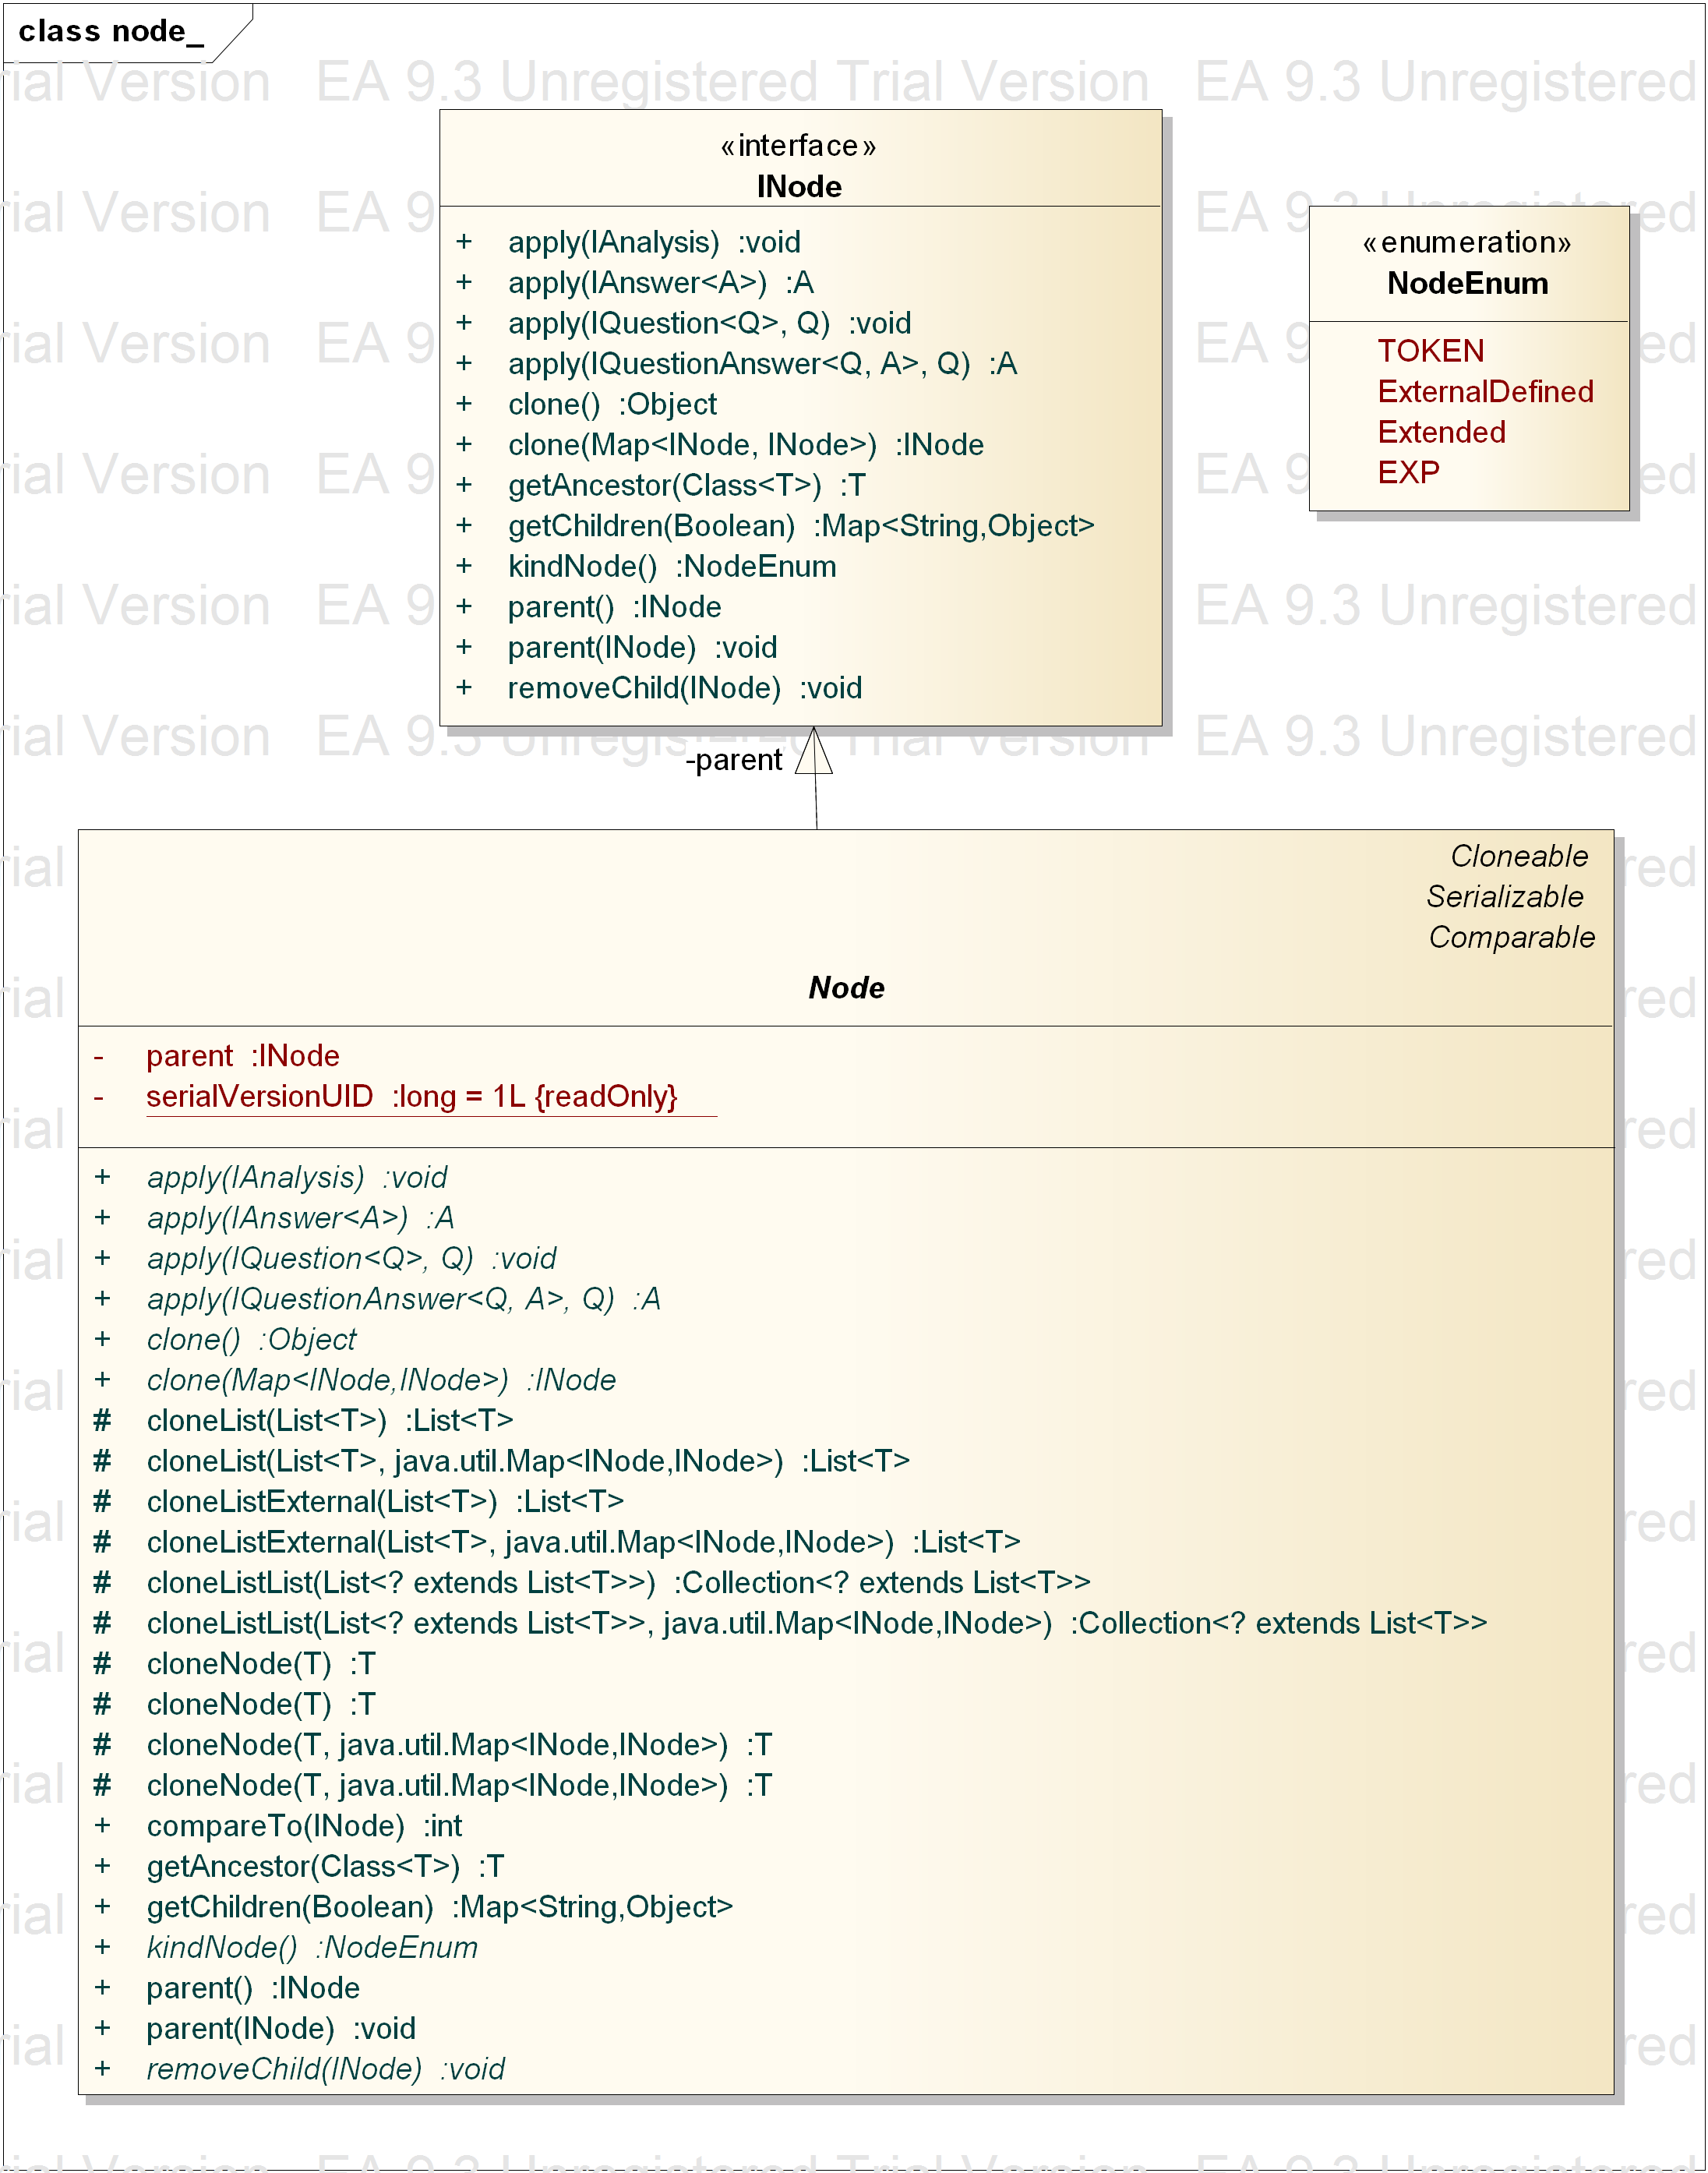
\includegraphics[width=0.8\textwidth]{figures/base_node}
\caption{Base node package}
%\label{fig:awesome_image}
\end{figure}

\begin{figure}[htb]
\centering
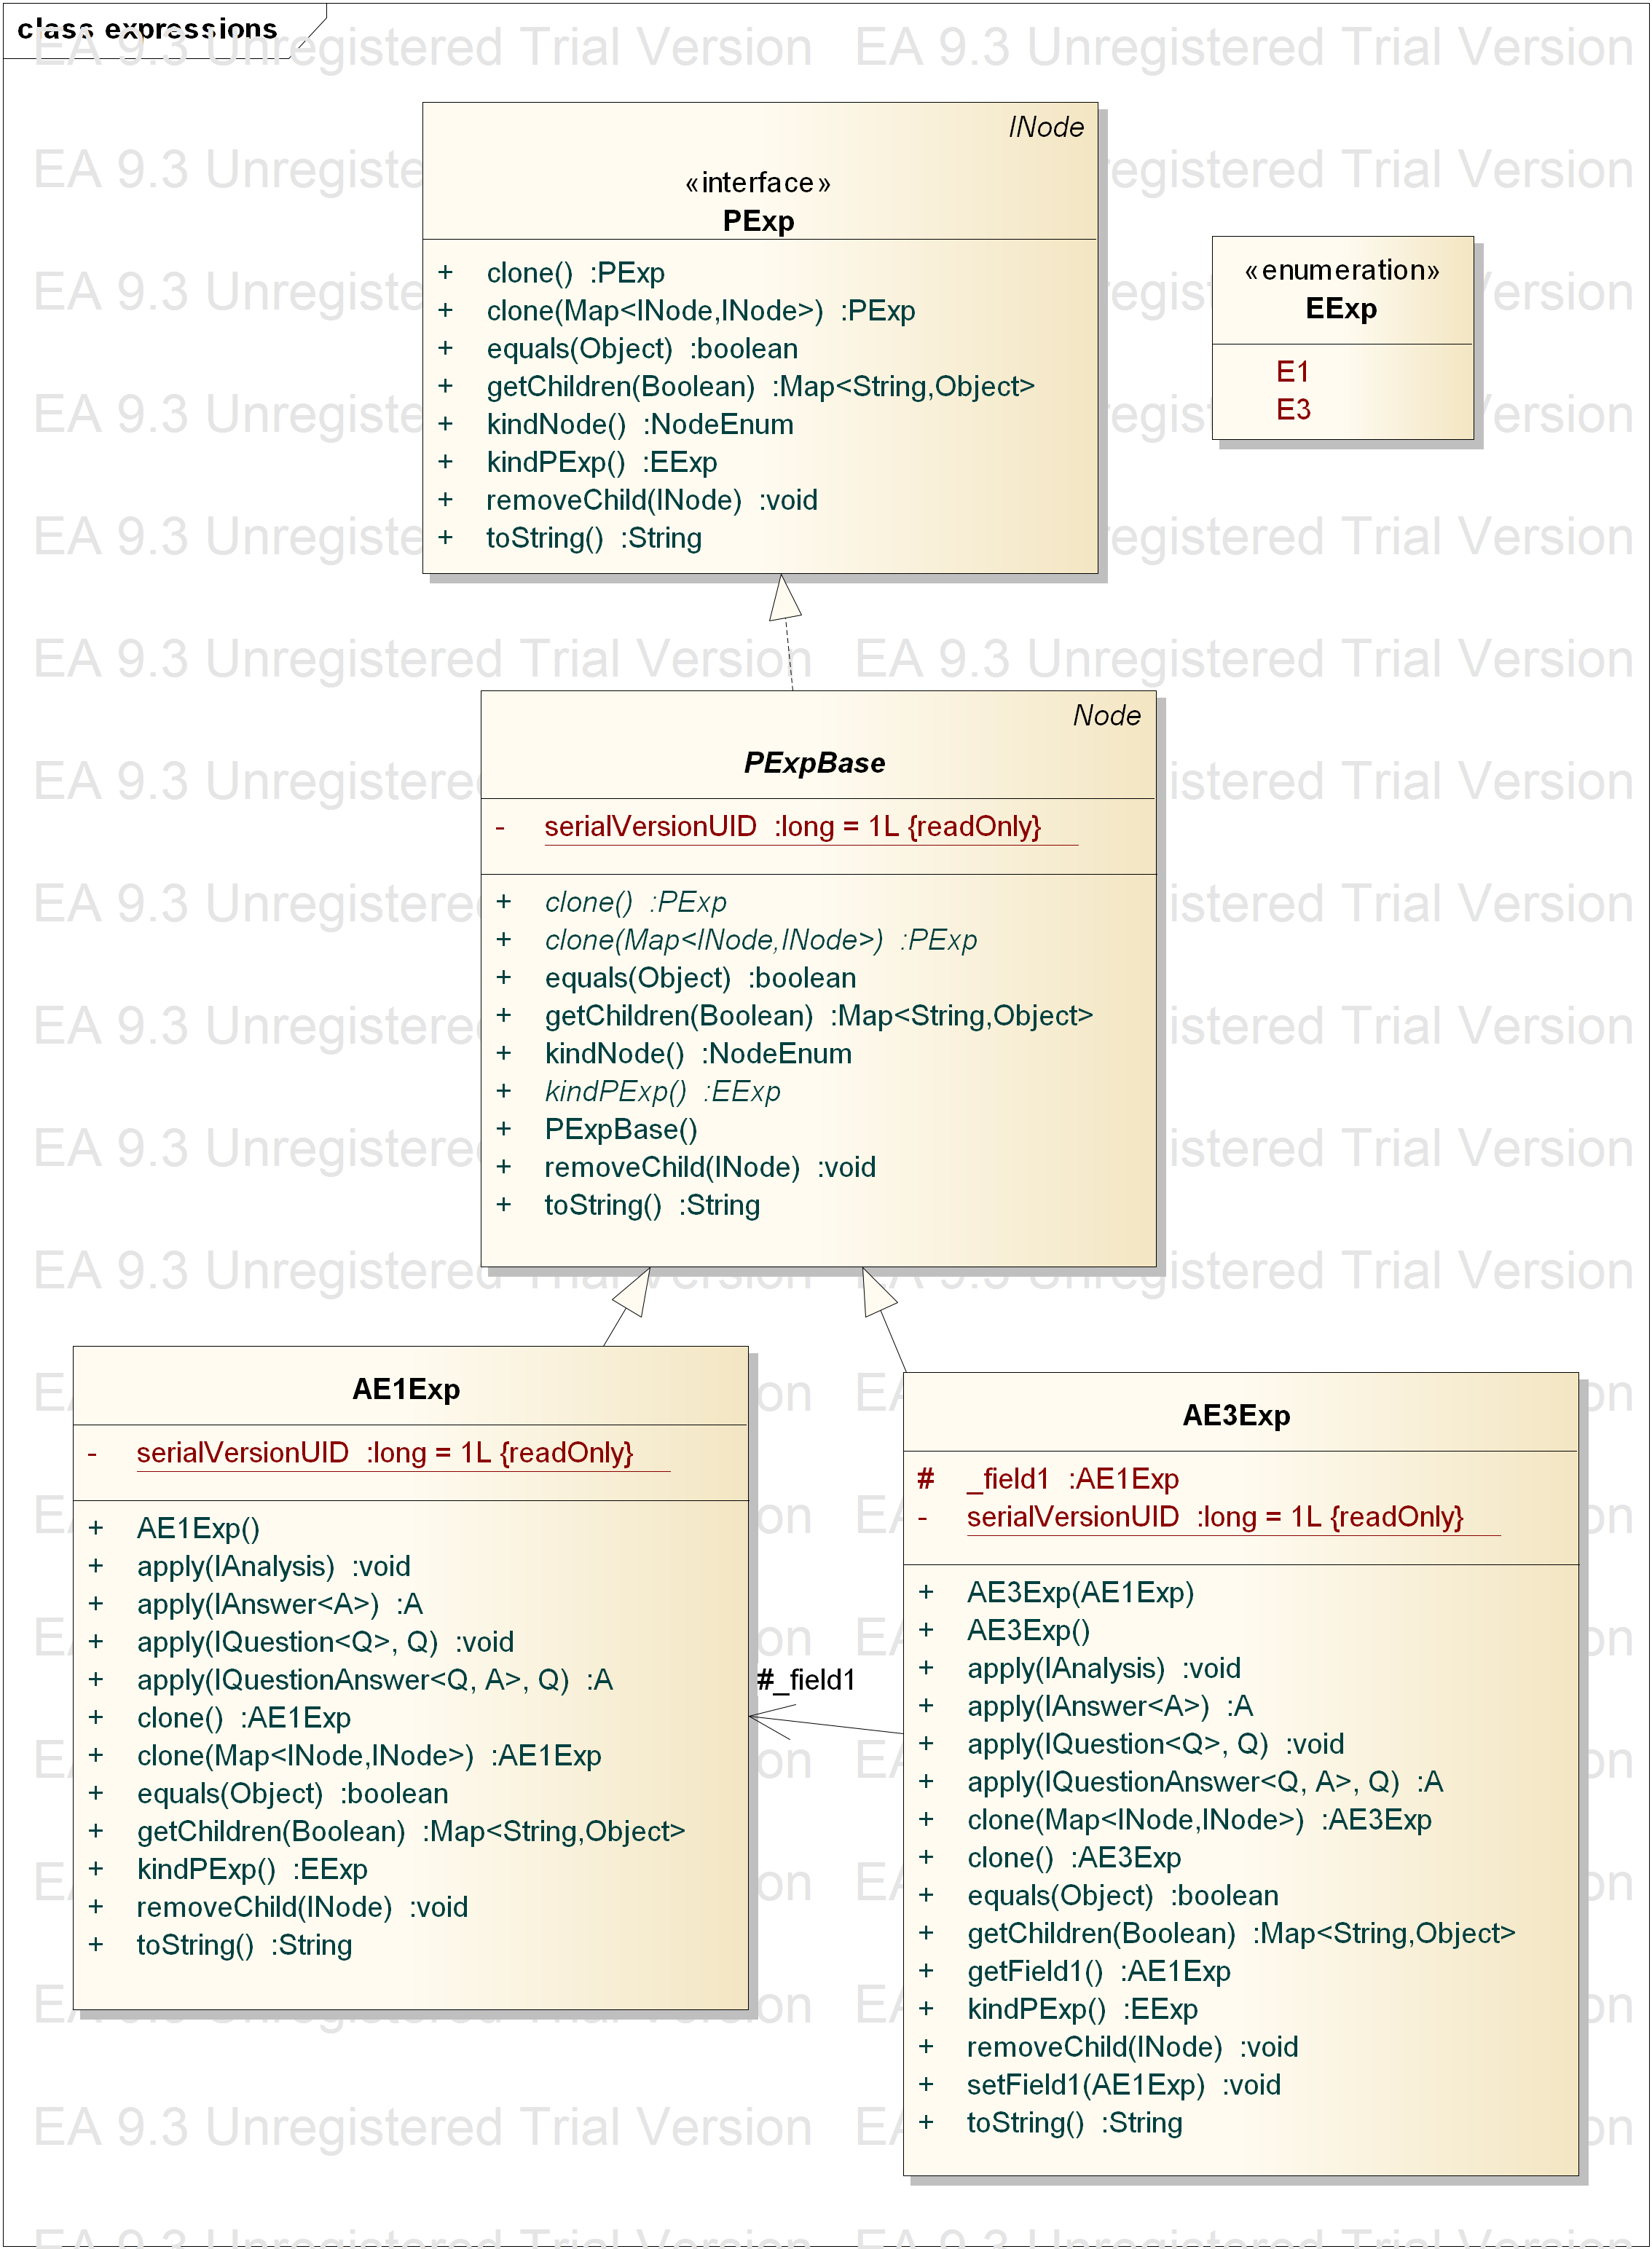
\includegraphics[width=0.8\textwidth]{figures/base_expressions}
\caption{Base expression package}
%\label{fig:awesome_image}
\end{figure}

\begin{figure}[htb]
\centering
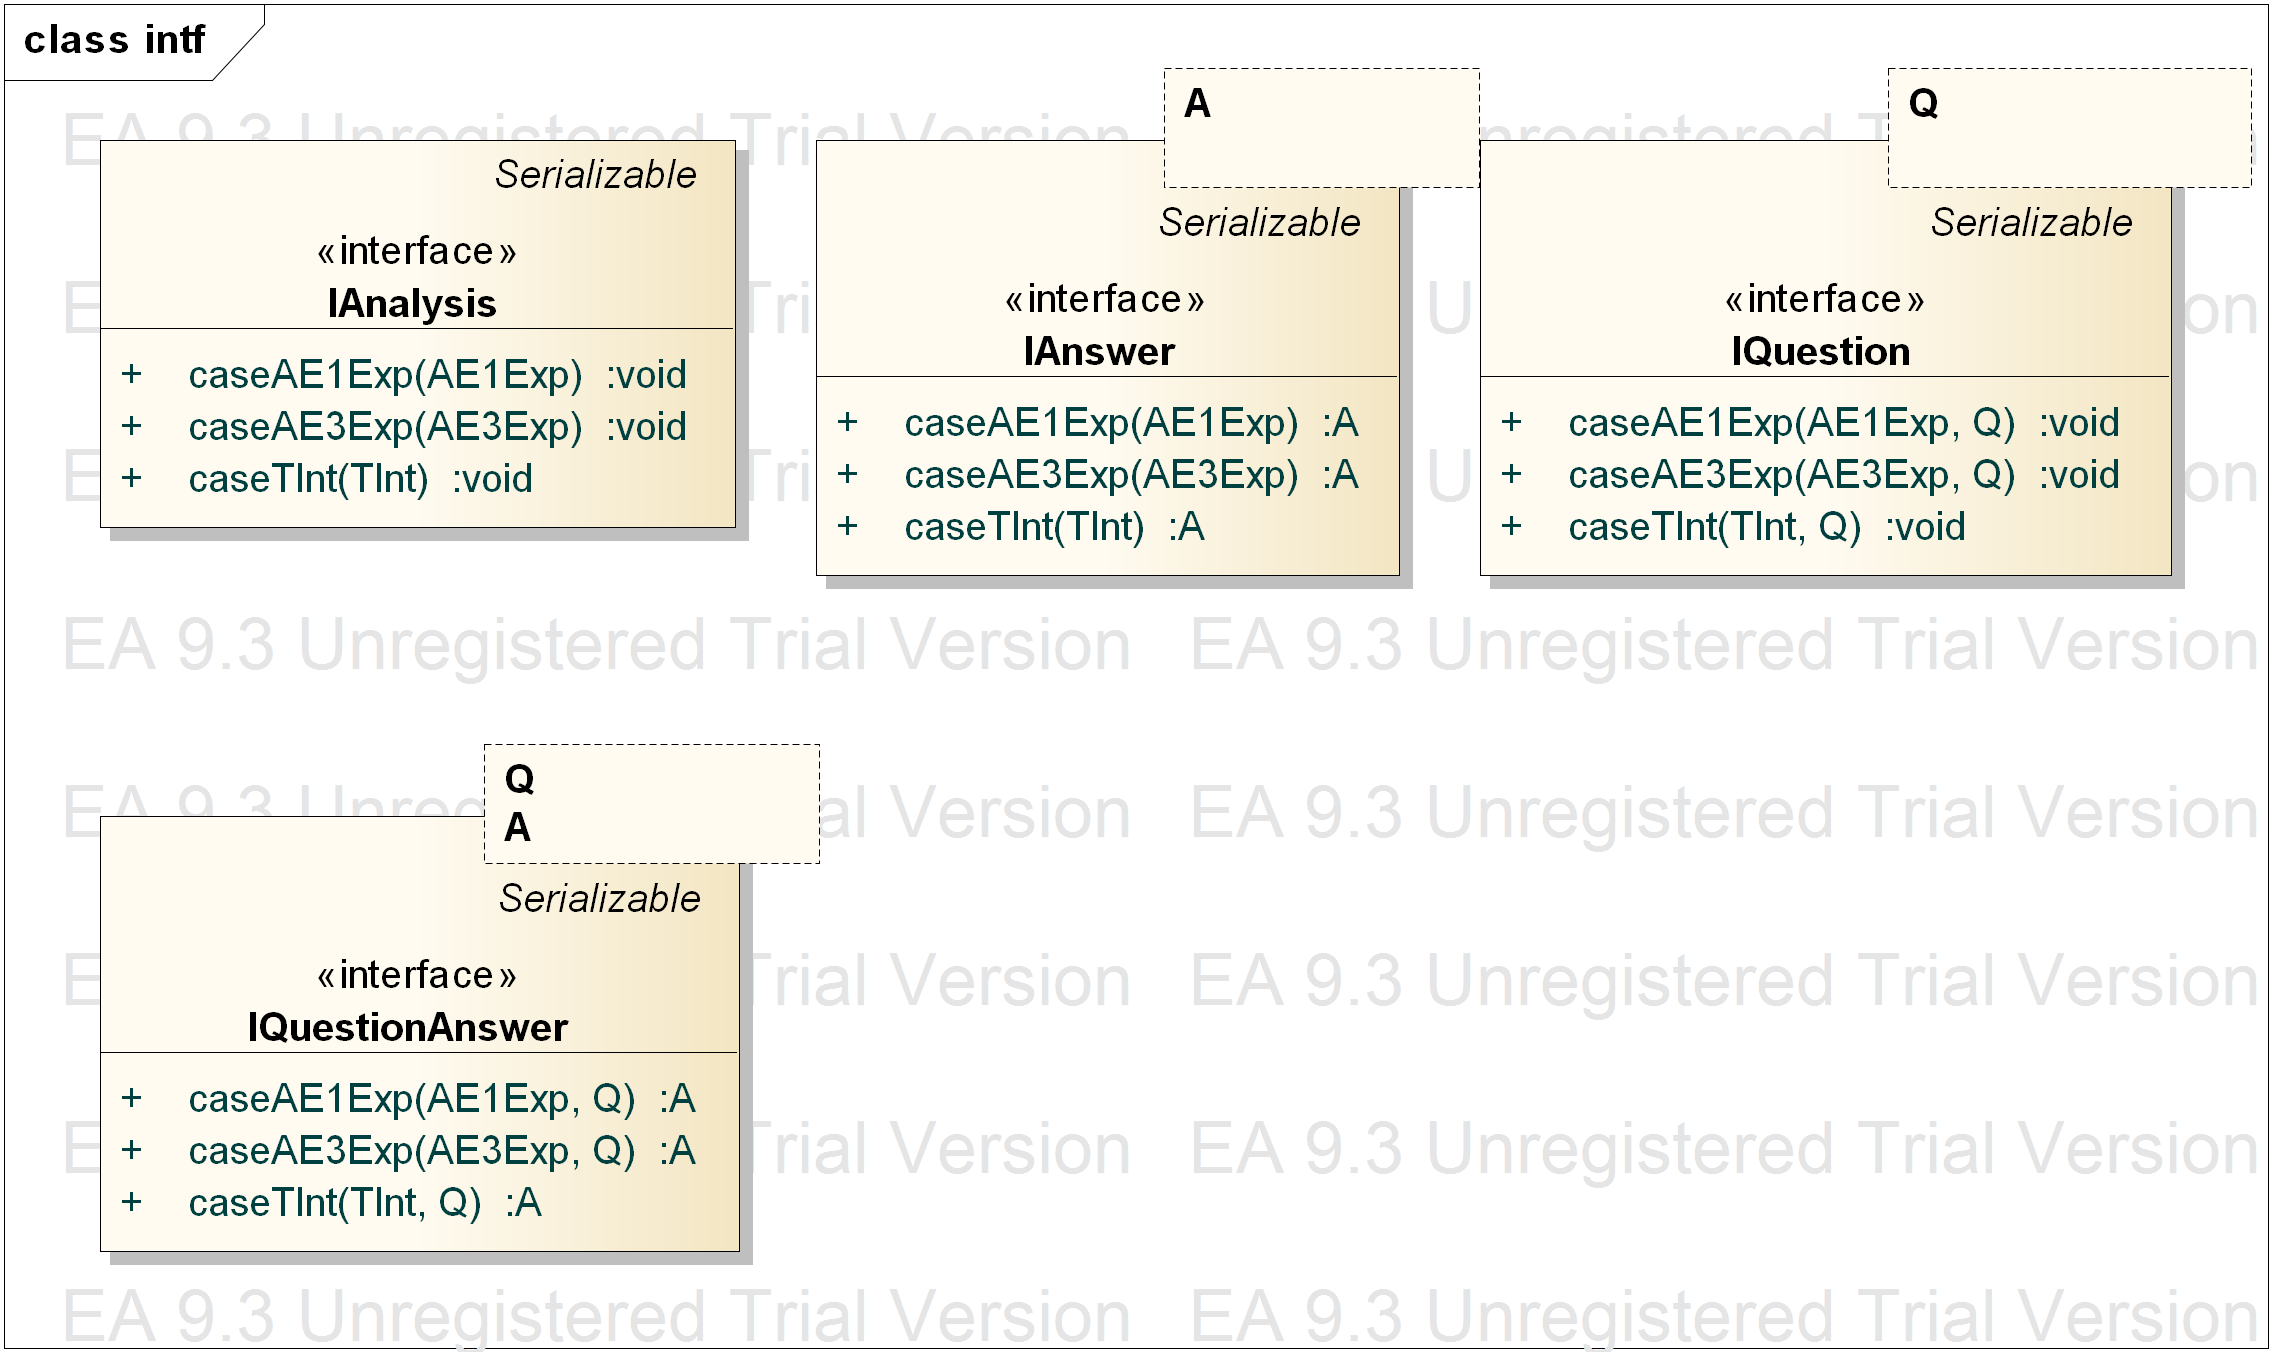
\includegraphics[width=0.8\textwidth]{figures/base_analysis_interfaces}
\caption{Base analysis interfaces package}
%\label{fig:awesome_image}
\end{figure}

\section{Extended}

\begin{figure}[htb]
\centering
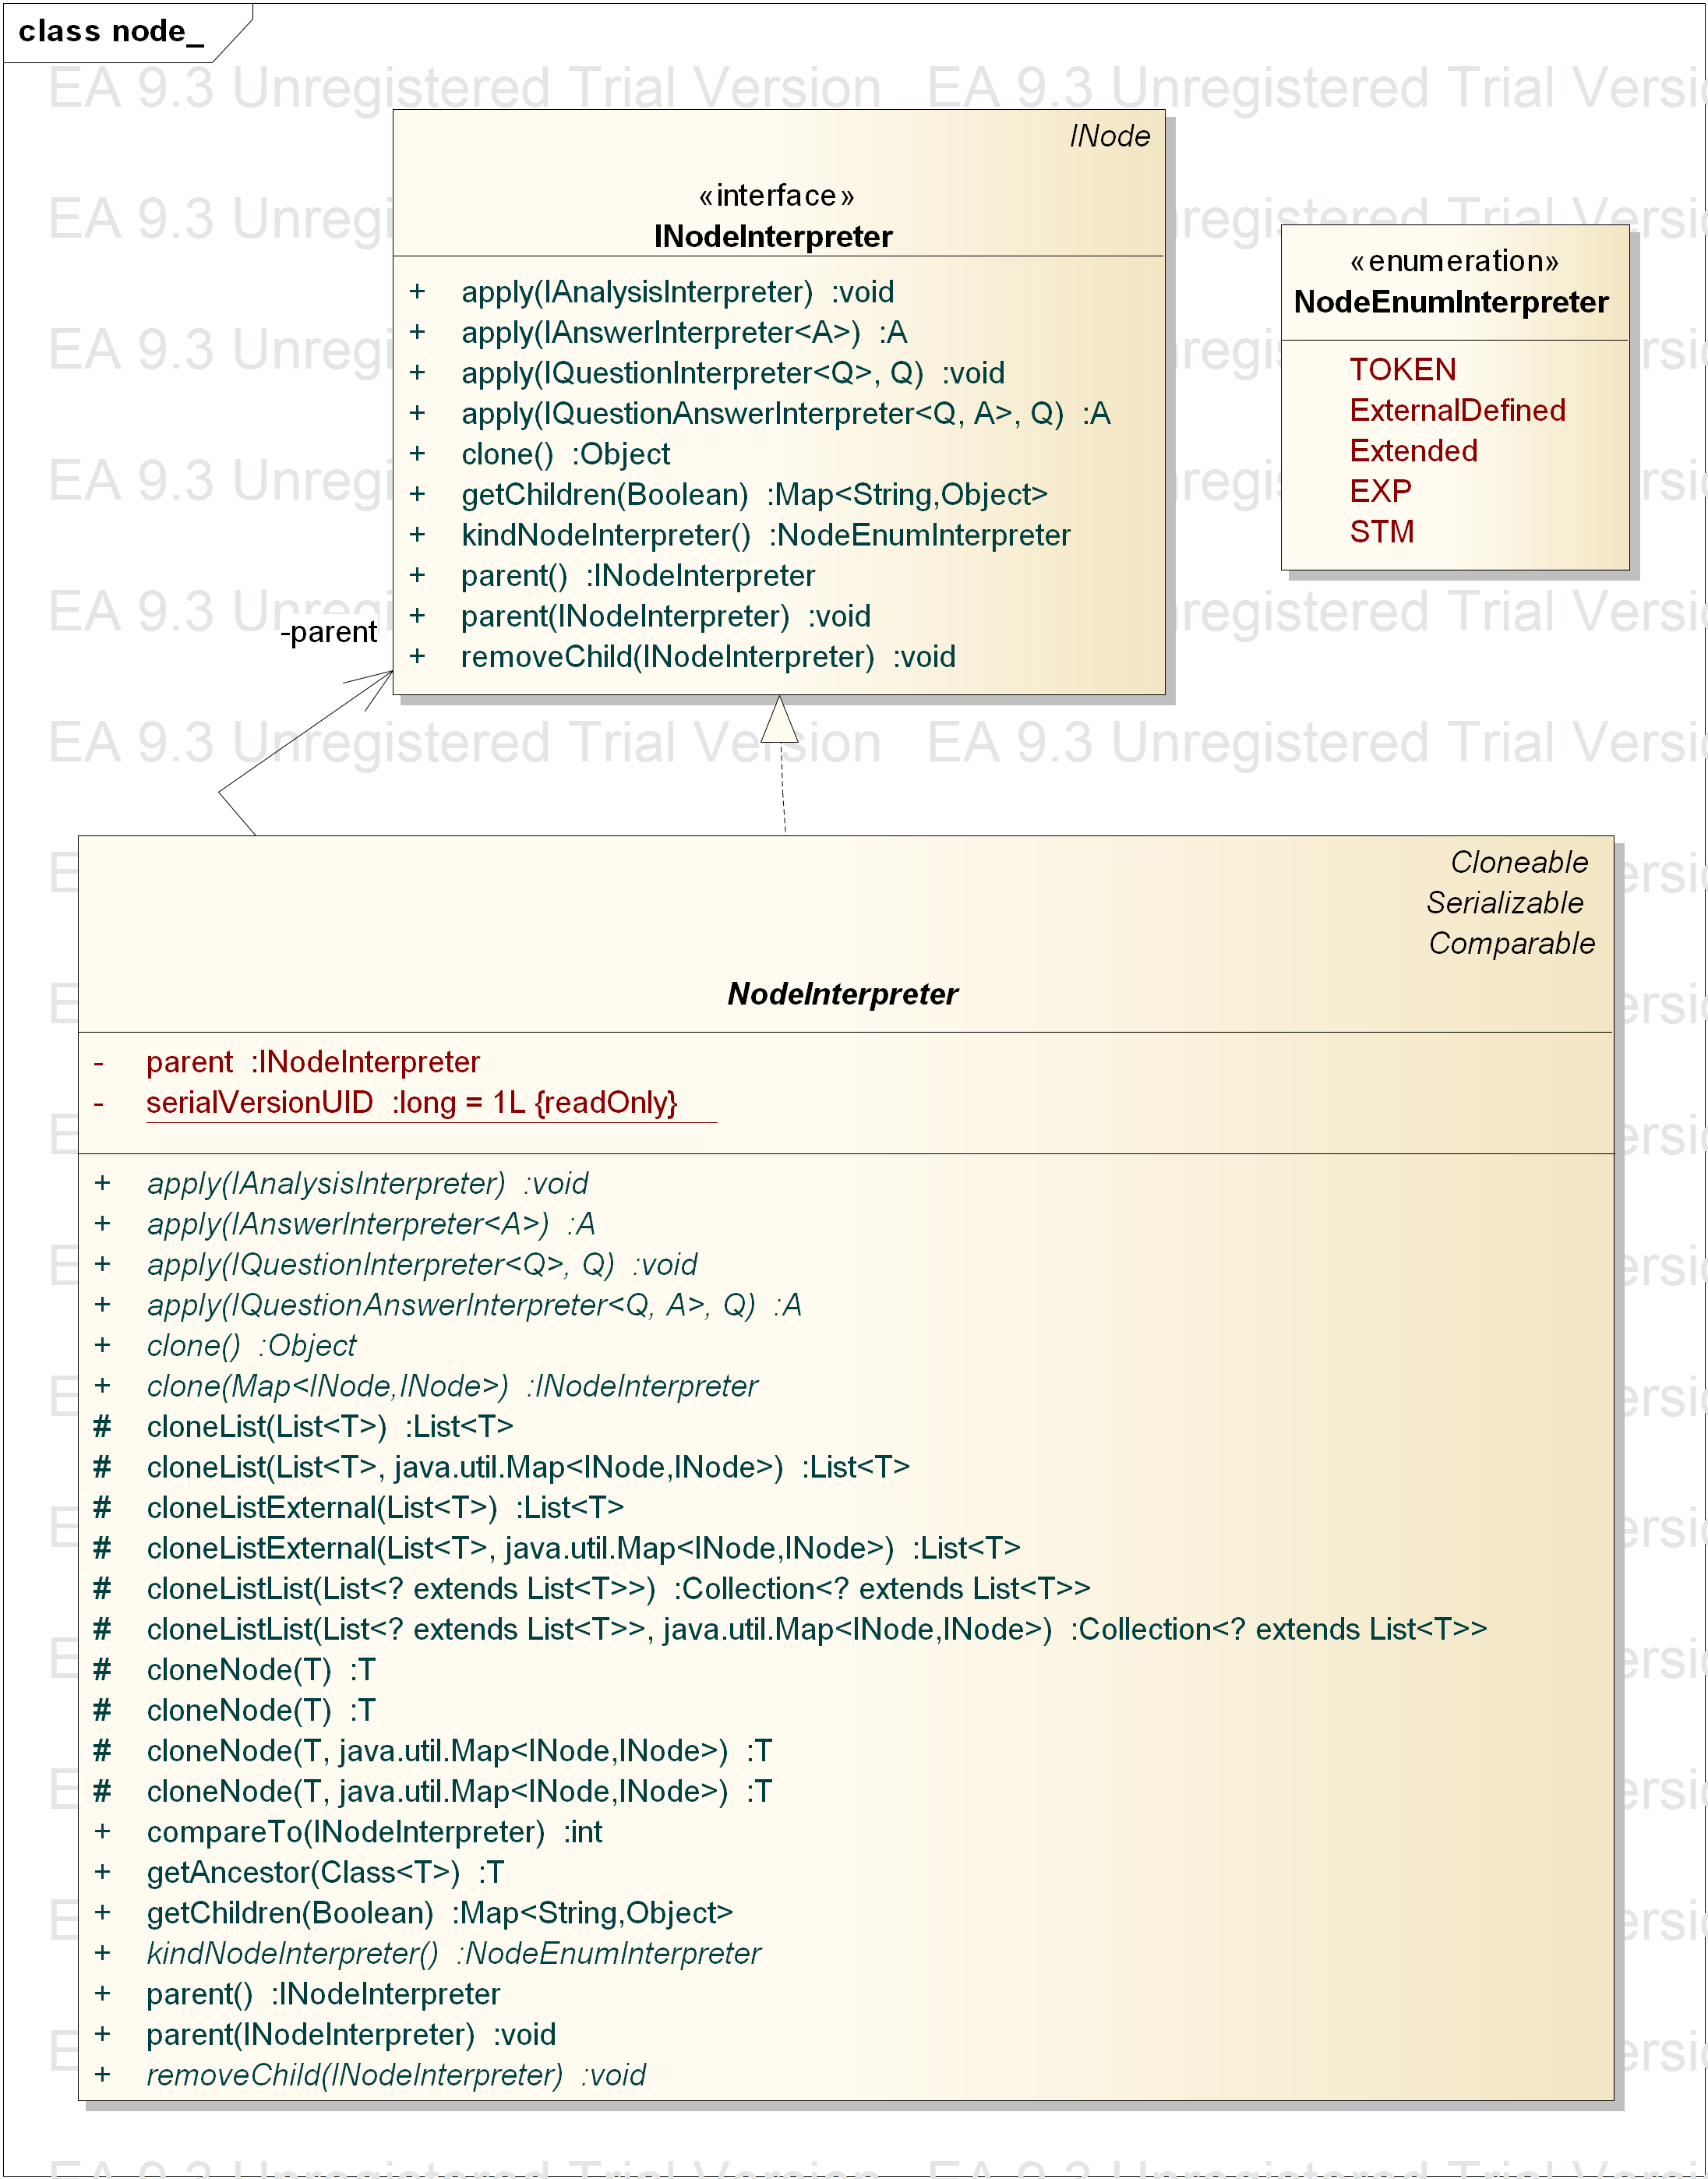
\includegraphics[width=0.8\textwidth]{figures/extended_node}
\caption{Extended node package}
%\label{fig:awesome_image}
\end{figure}

\begin{figure}[htb]
\centering
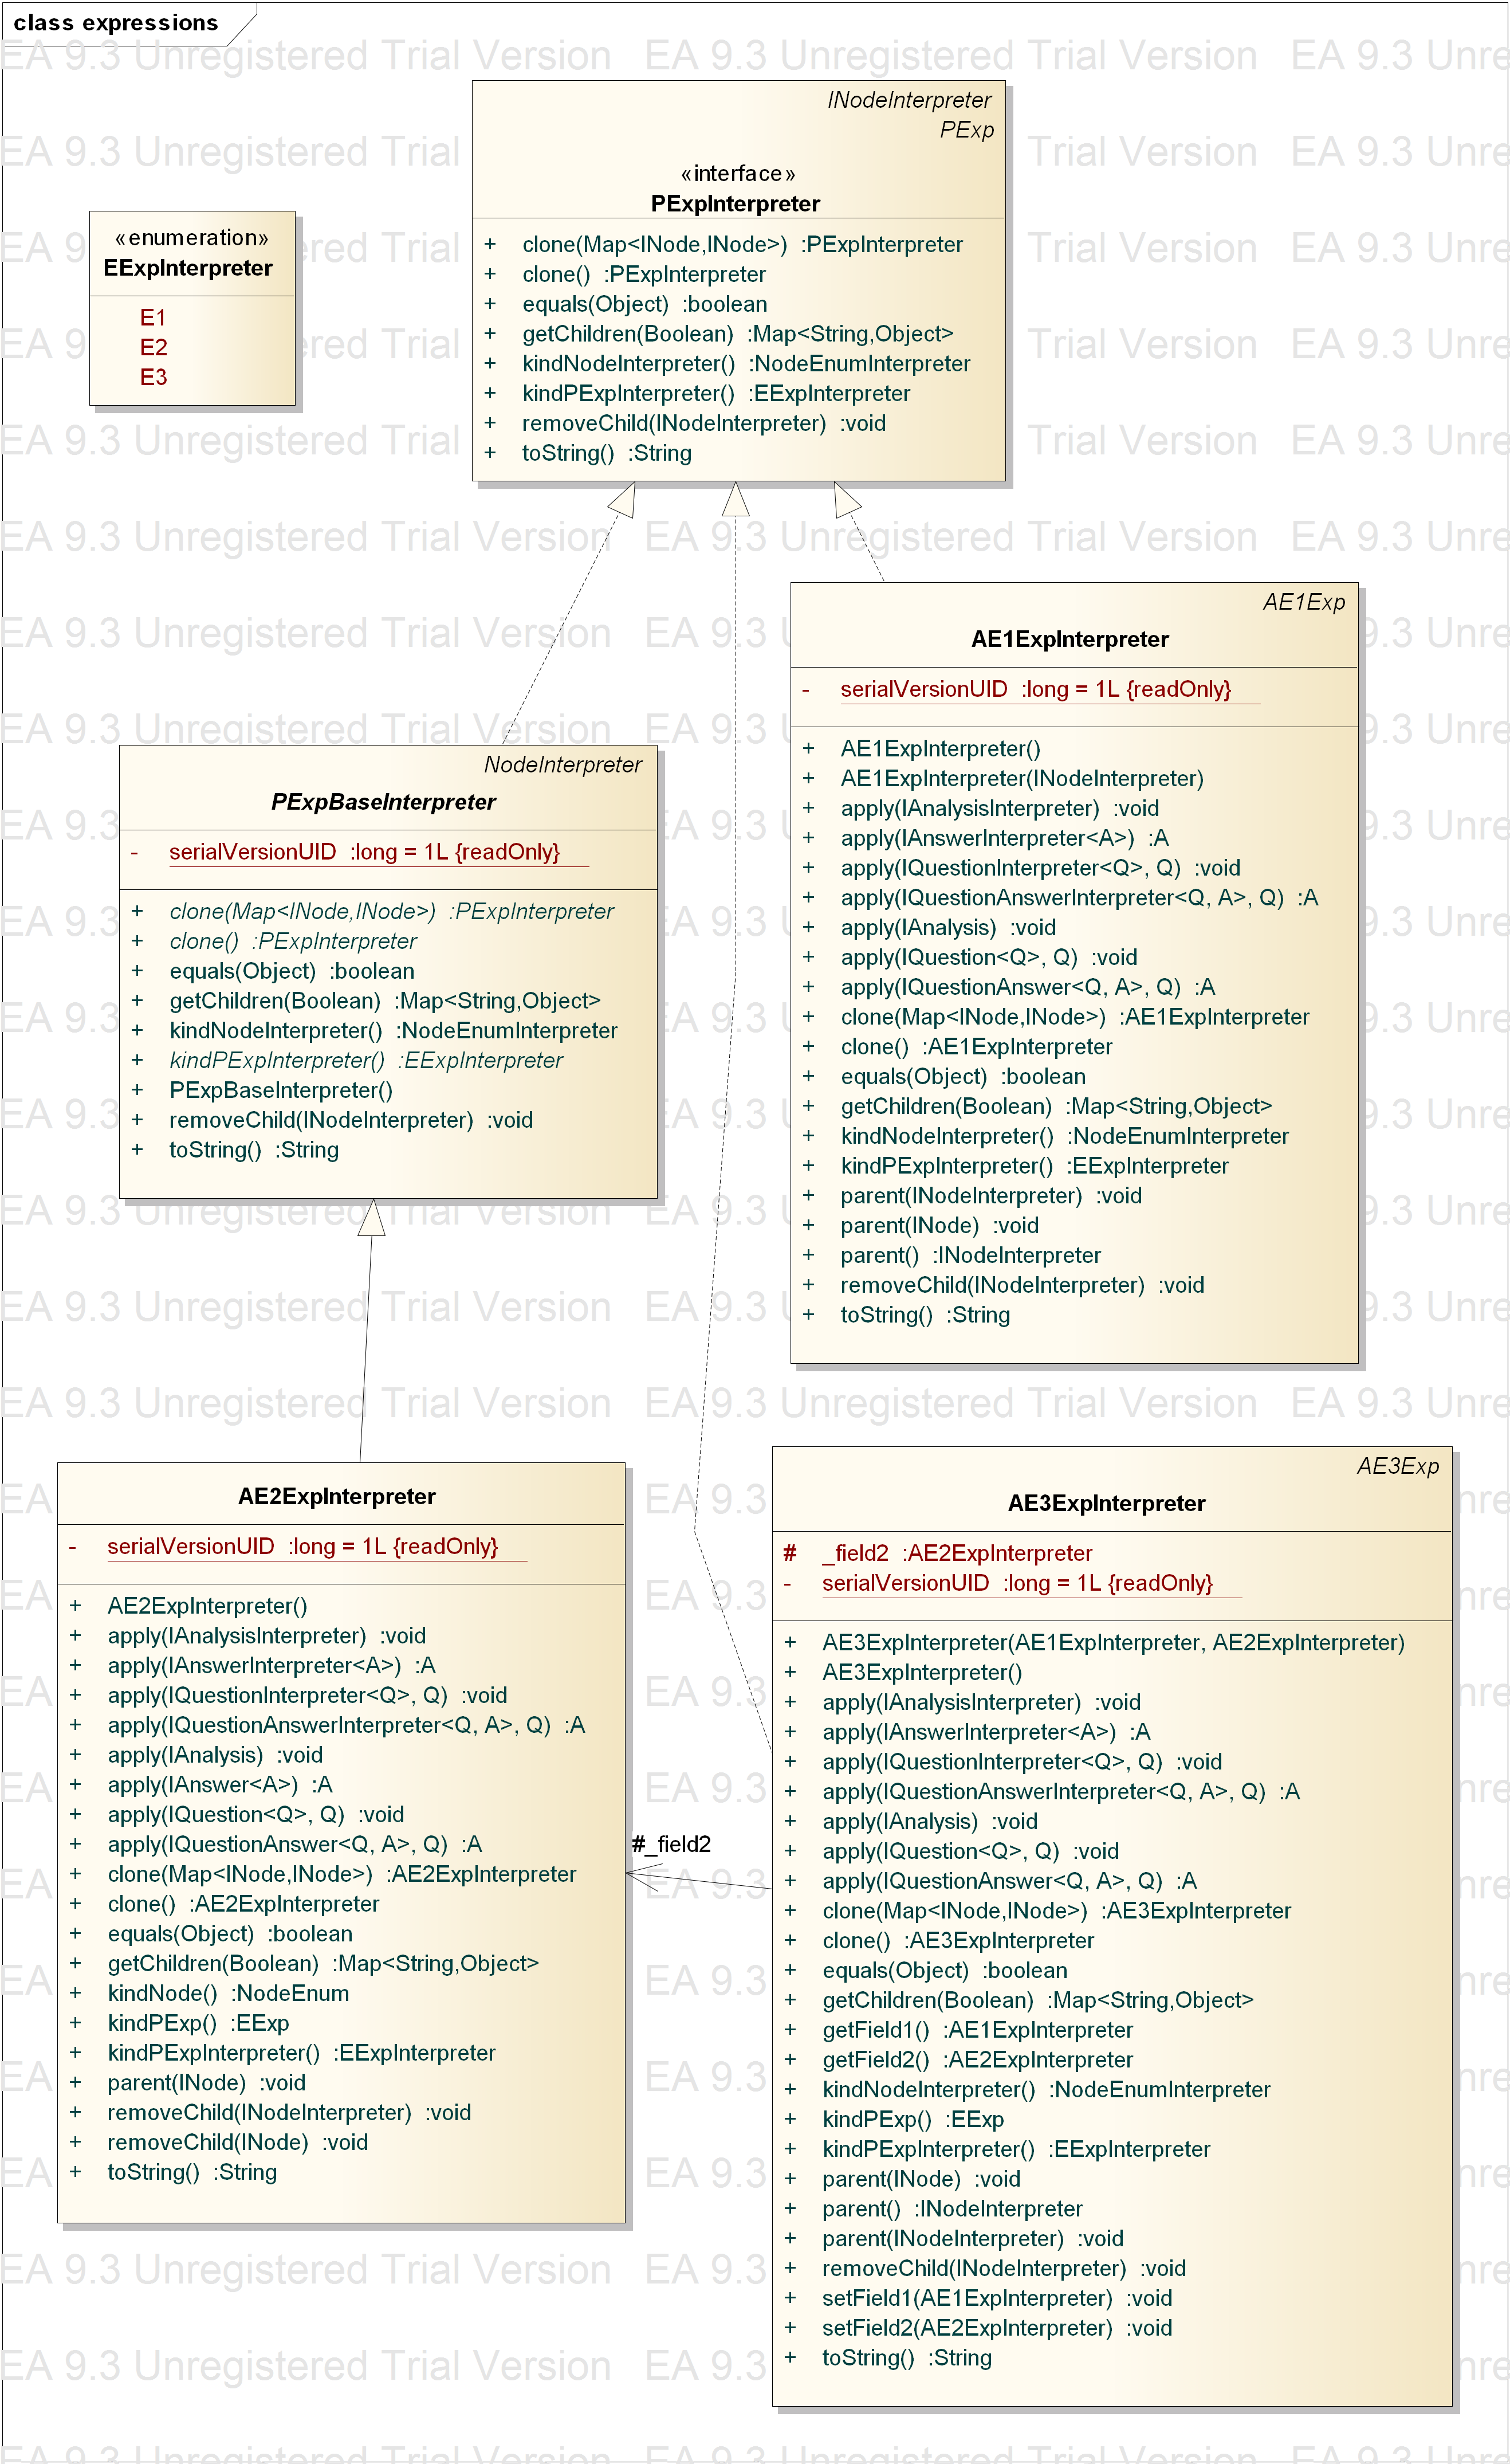
\includegraphics[width=0.8\textwidth]{figures/extended_expressions}
\caption{Extended expressions package}
%\label{fig:awesome_image}
\end{figure}

\begin{figure}[htb]
\centering
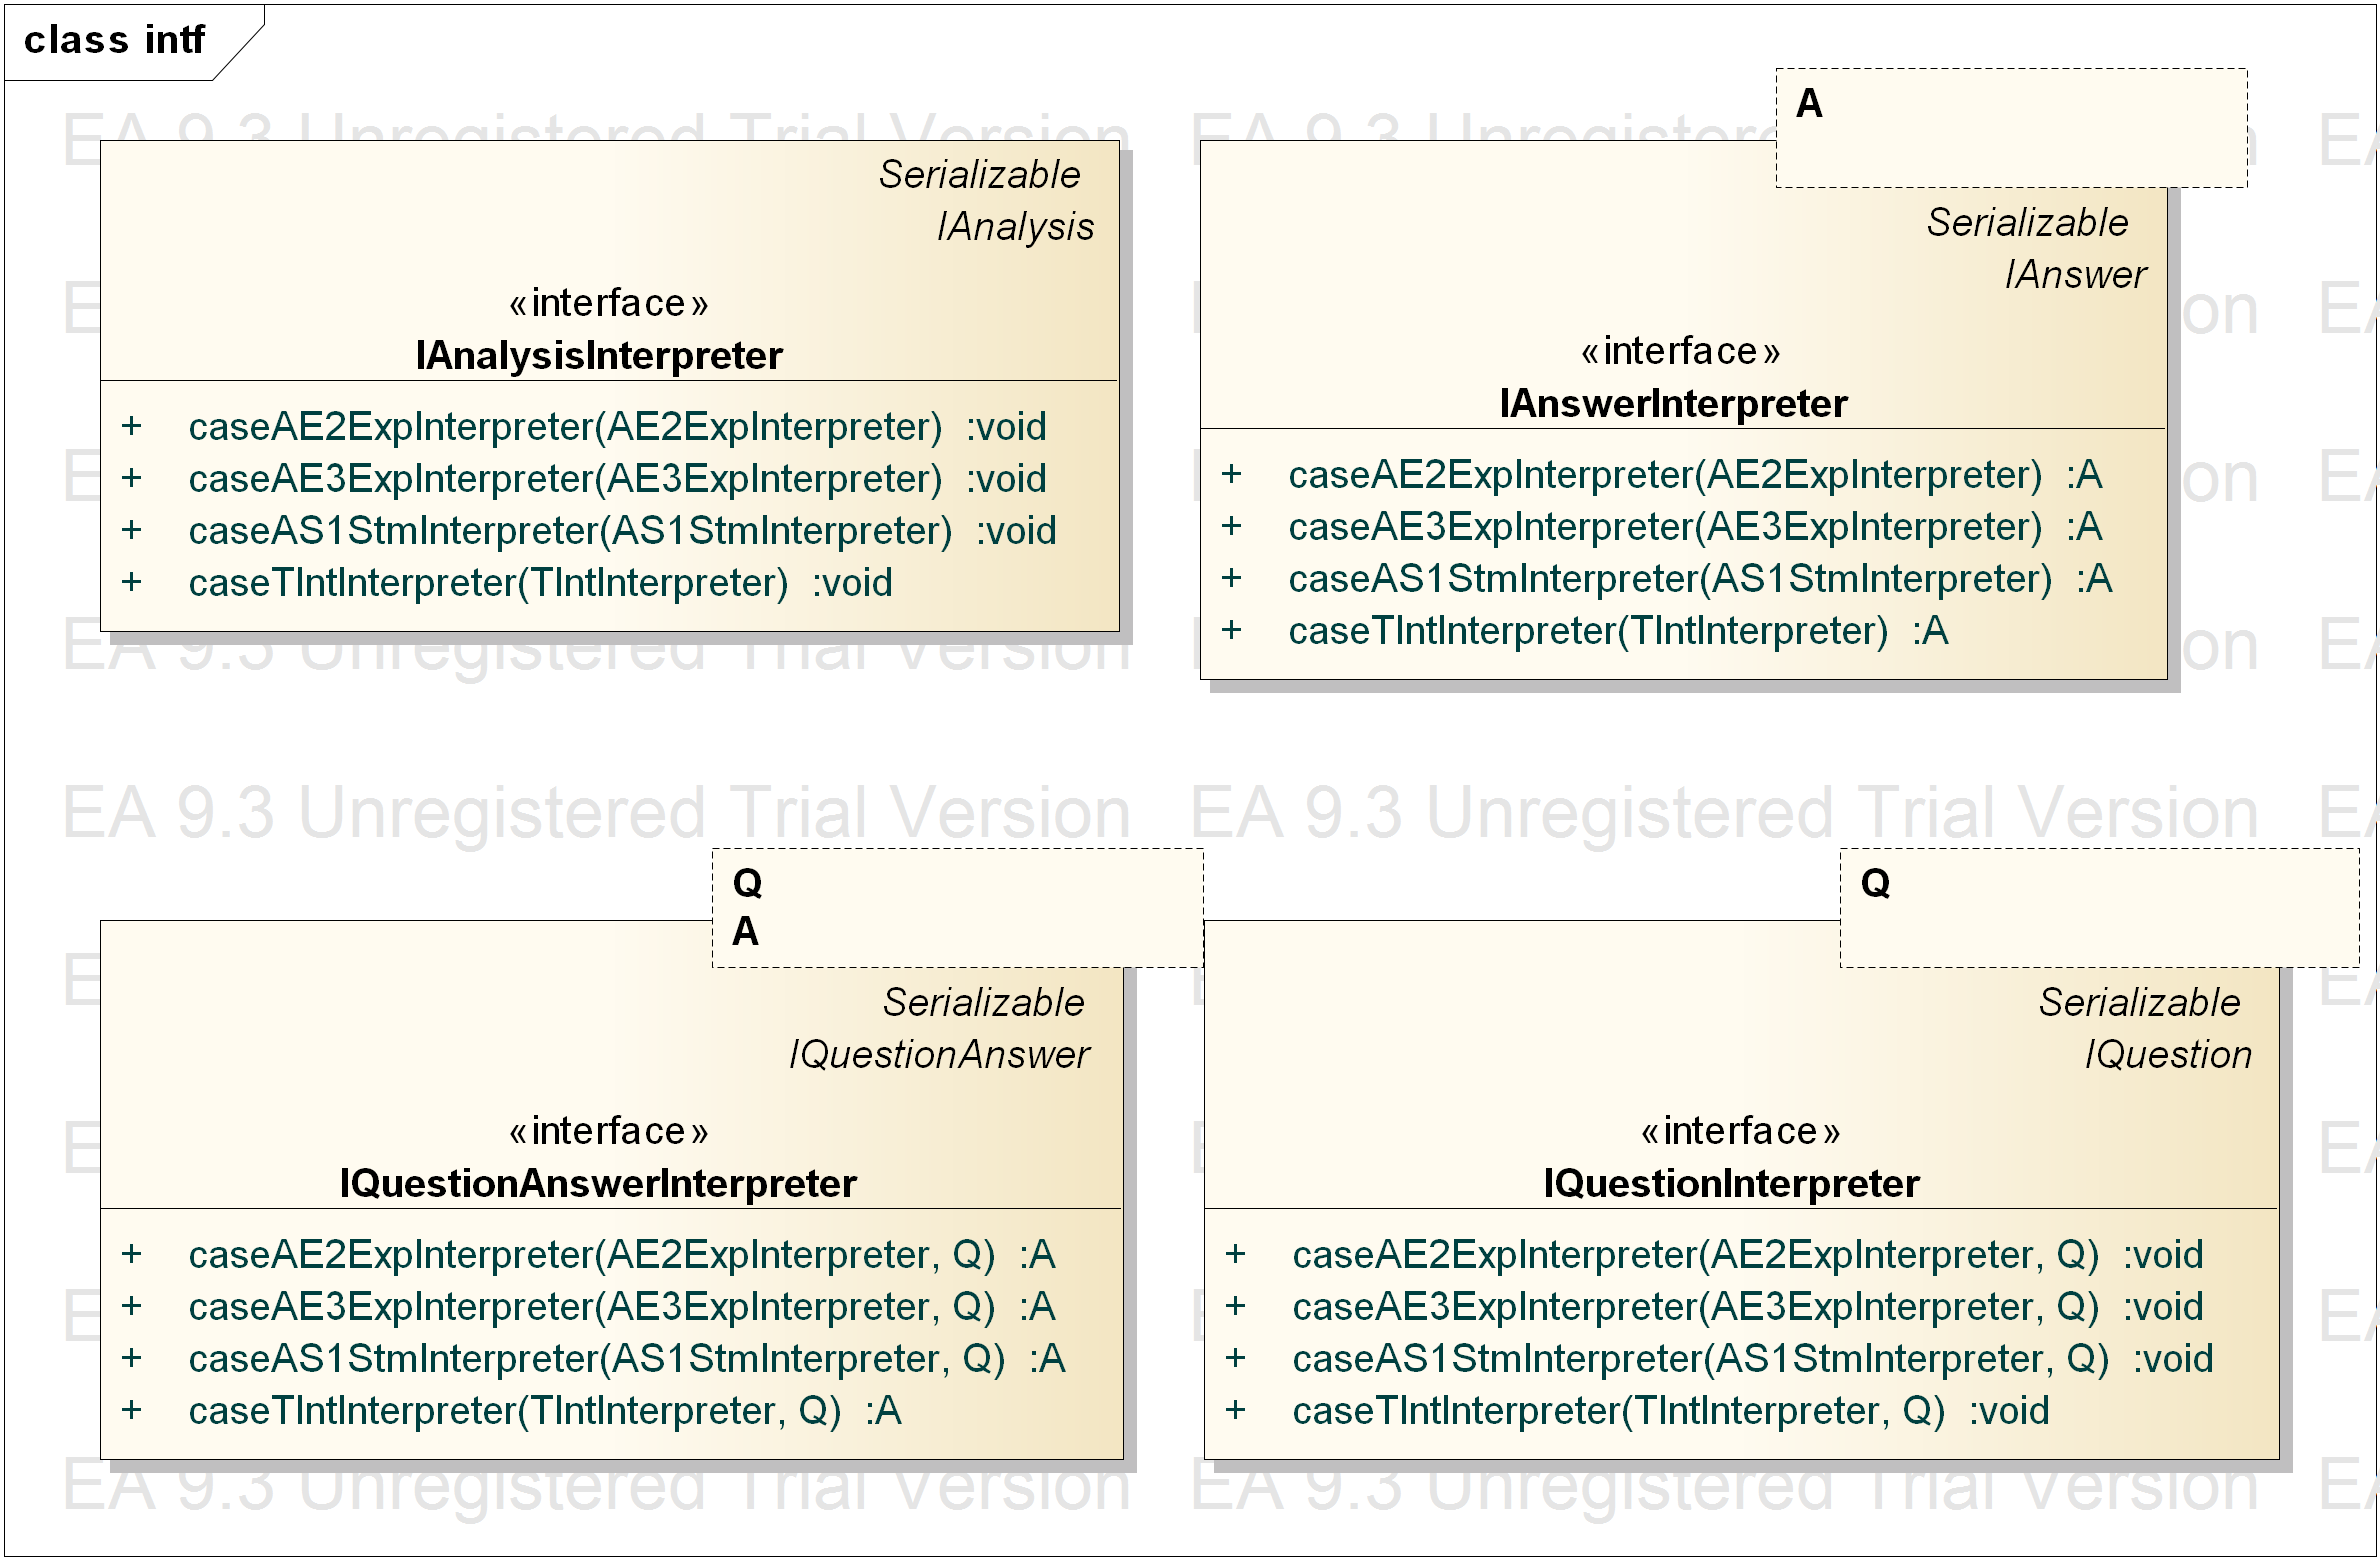
\includegraphics[width=0.8\textwidth]{figures/extended_analysis_interfaces}
\caption{Extended analysis interfaces package}
%\label{fig:awesome_image}
\end{figure}

\begin{figure}[htb]
\centering
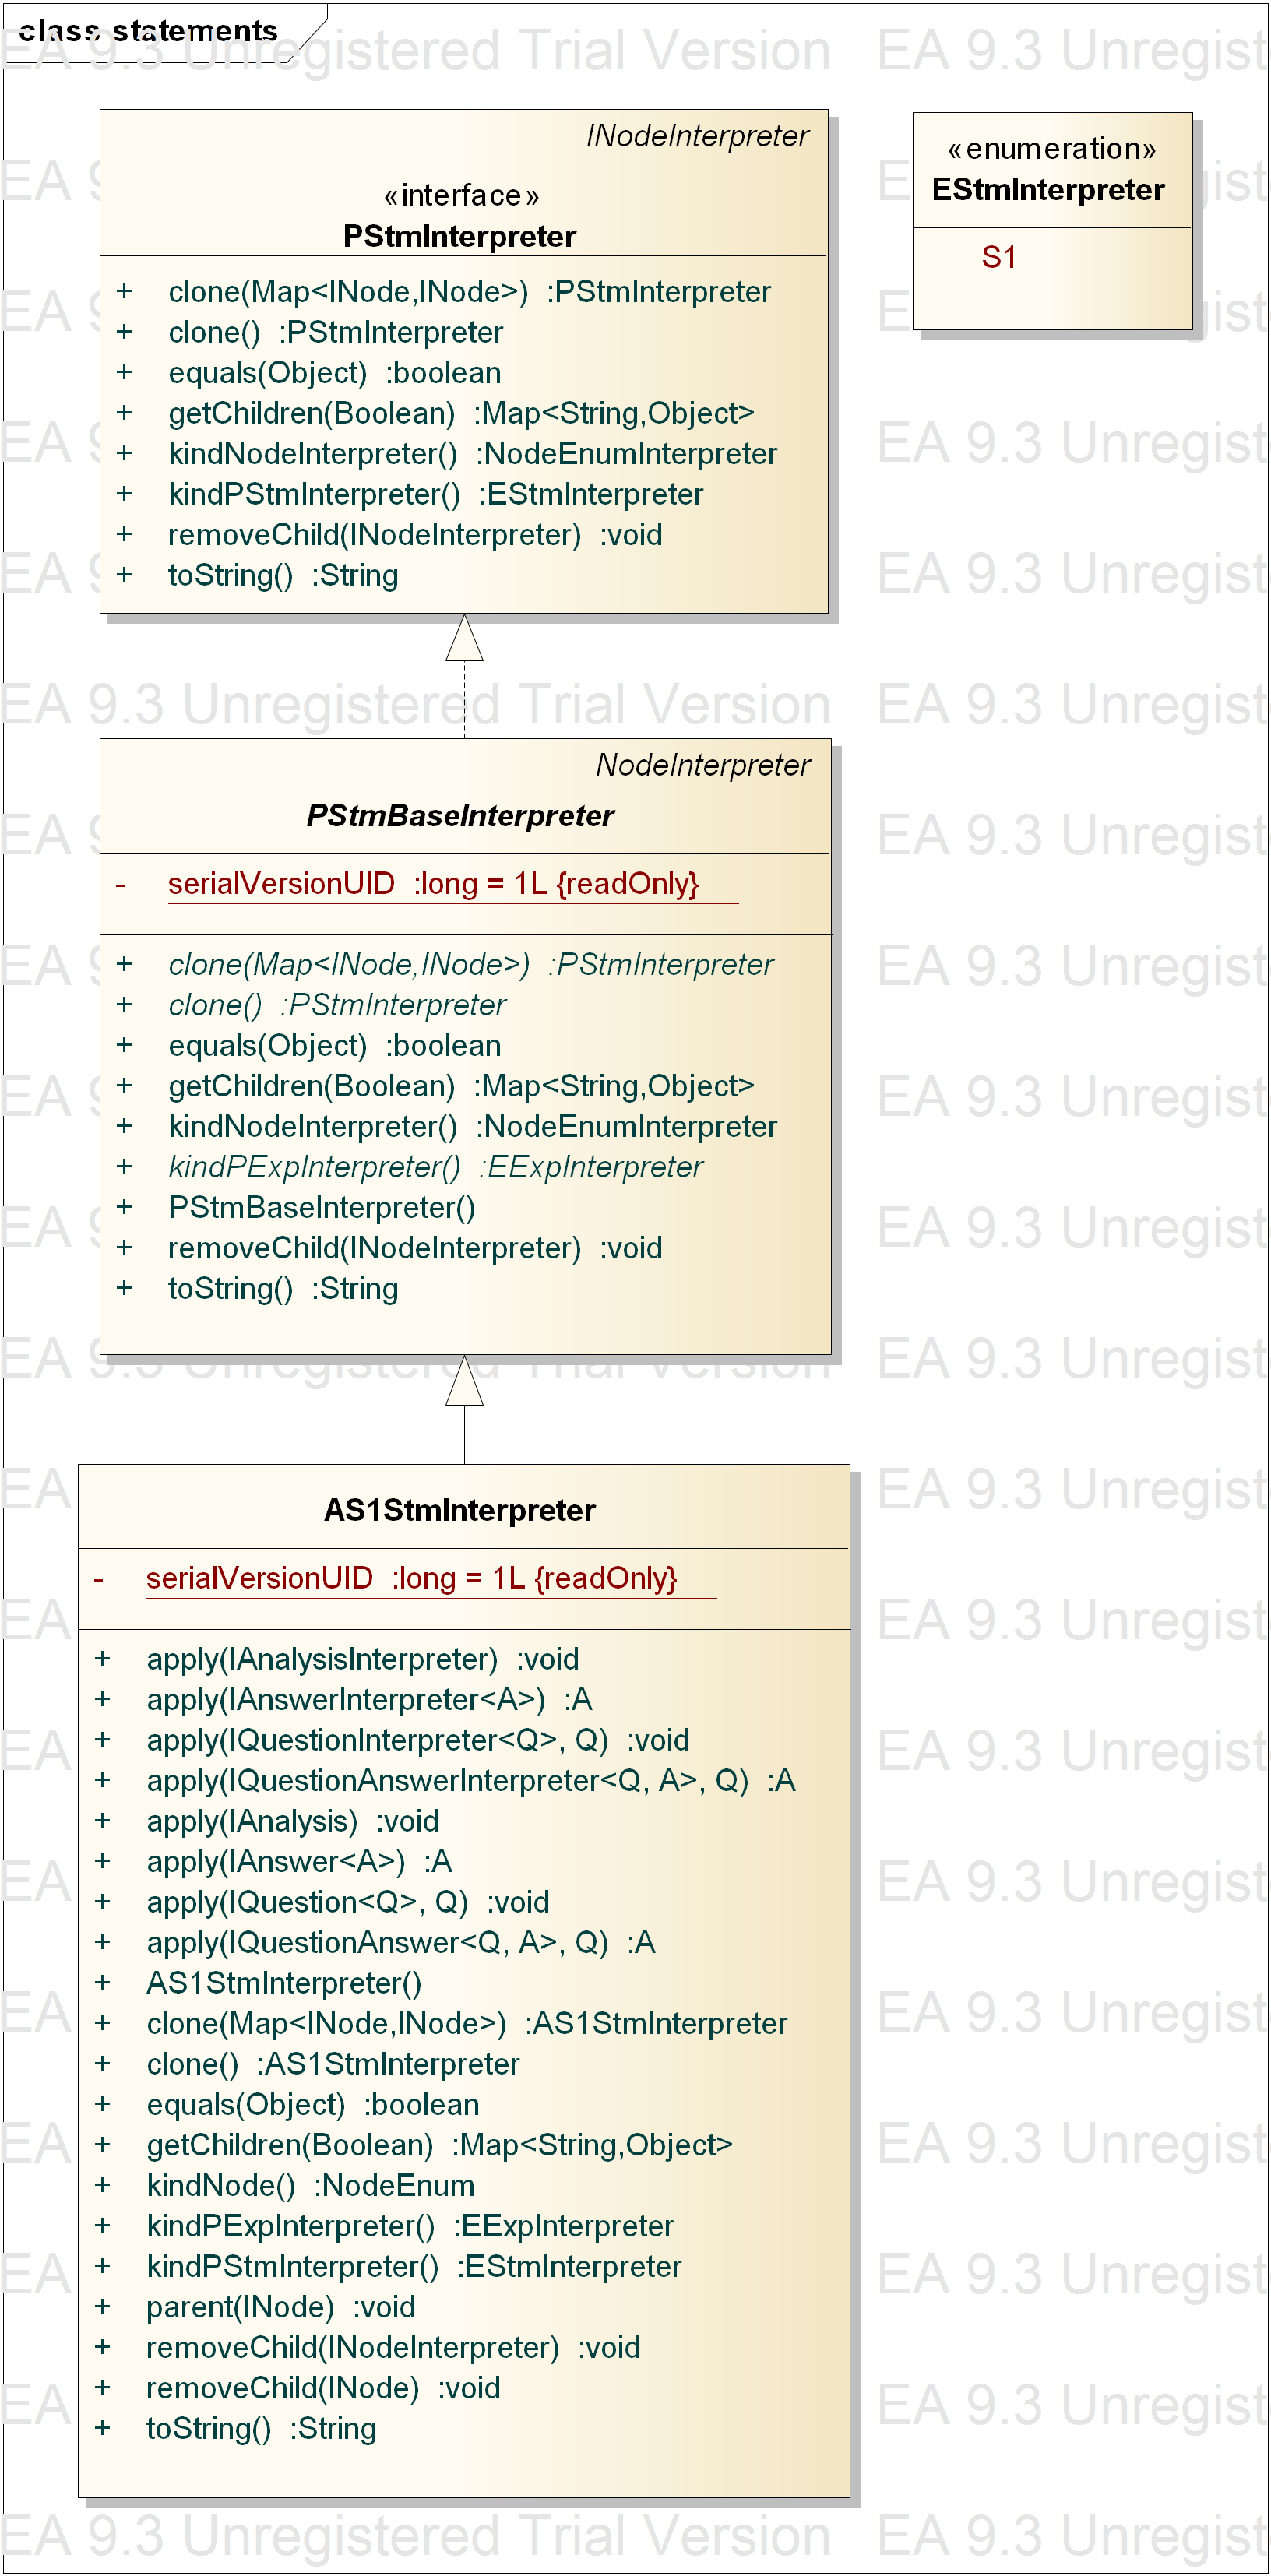
\includegraphics[width=0.8\textwidth]{figures/extended_statements}
\caption{Extended statements  package}
%\label{fig:awesome_image}
\end{figure}

\section{Extended AST Test Class}

\lstinputlisting[language=java,tabsize=2,basicstyle=\ttfamily\footnotesize,showspaces=false,showstringspaces=false,showtabs=false,keywordstyle=\color{blue},        commentstyle=\color{dkgreen}, stringstyle=\color{mauve}]{example/src/TestCase1.java}

\chapter{Challanges}

\begin{itemize}
\item Tree consistency
\item Tree automated analysis; visit in decent order
\item Generating a tree to replace OO developed classed. Dificult because of functionality embedded in the classes where 1,2,4 super classes all might override some methods.
\item Caching: converting a program which does OO caching/linking to use a generated tree. Not easy, solutions:
	\begin{itemize}
		\item Hashmap
		\item Add custum graph fields to the tree. Nodes in a graph field would be different because they are not a child of the node when are attached to. In relation to tree fields which can only have one parent and thus needs to disconnect from their previously attached parent before moving to a new,
	\end{itemize}
\item Handling OO embeded functions outside a tree. Developing assistants to handle public/private functions from OO tree. The difficulty is to keep the hierarchy intact.
\item Display: For debugging it is important to have a decent toString of a tree, two solutions:
	\begin{itemize}
		\item Generated toString including all fields of a node and it name.
		\item Custom toString. Since a tree might represent (to some extend) the syntax of a language a toString representation close to the real syntax might be prefered. One solution would be to add a way to define the toString method of nodes based on their fields and strings plus possibly allowing external java methods to be called for more advanced display functions.
	\end{itemize}
\end{itemize}

\end{document}


